\chapter{Unit 1: Astronomy}

\section{Episode 1: Standing up in the Milky Way}
\begin{enumerate}
    \item What is responsible for creating wind and keeping everything in the solar system in its clutches?
    \begin{itemize}
        \item Gravity
    \end{itemize}
    \item What lies between Mars and Jupiter?
    \begin{itemize}
        \item The asteroid belt
    \end{itemize}
    \item What had to be invented before we could discover Saturn and Neptune
    \begin{itemize}
        \item The telescope
    \end{itemize}
    \item What is the name of the spacecraft that has travelled the farthest away from Earth?
    \begin{itemize}
        \item Voyager 1
    \end{itemize}
    \item What is the Oort Cloud?
    \begin{itemize}
        \item A cloud of billions of ice planetesimals surrounding the sun 
    \end{itemize}
    \item What is the "addresss" of Earth in the cosmos?
    \begin{itemize}
        \item Earth, Solar System, Orion Arm, Milky Way, Local Group, Virgo Supercluster, Laniakea Supercluster, Universe
    \end{itemize}
    \item Who was able to prove Giordano Bruno right 10 years after his death?
    \begin{itemize}
        \item Galileo
    \end{itemize}
\end{enumerate}

\section{Episode 4: A Spacetie Odyssey}
\begin{enumerate}
    \item Why do we see the Sun rise before it is over the horizon?
    \begin{itemize}
        \item Because Earth's atmosphere refracts the Sun's image
    \end{itemize}
    \item How far away is Neptune from Earth (in light hours)?
    \begin{itemize}
        \item 4.17 light hours
    \end{itemize}
    \item Using the idea of how fast light travels, how do scientists know our universe is older than 6500 years?
    \begin{itemize}
        \item We know that there are objects farther than 6500 light year away from Earth. 
    \end{itemize}
    \item Why does no one know what happened before the Big Bang?
    \begin{itemize}
        \item No evidence survived
    \end{itemize}
    \item How long after the Big Bang did it take for stars to form?
    \begin{itemize}
        \item Millions of years
    \end{itemize}
    \item What did Einstein call the “rules” that must be obeyed when traveling at high speeds?
    \begin{itemize}
        \item Principle of relativity
    \end{itemize}
\end{enumerate}

\section{Measuing the Universe}

\subsection{Some important constants}
The speed of light $c$:
\[
    c = 3.00 * 10^8\frac{m}{s} (3SD)
\]
The distance of a light year:
\[
    \text{A light year} = 9.4608 * 10^{15} m (3SD)
\]
The distance between \textcolor{red}{Earth} and \textcolor{red}{Sun} refers to the \textit{Astronomicial Unit (AU)}
\[
    AU = 1.4958 * 10^{11}m (3SD)
\]
One Parsec is \textcolor{red}{3.26} light years \[
\text{Parsec} = 3.0824 * 10^{16}m (3SD)
\]

\subsection{Unit Conversion}
\begin{blueblock}
\begin{example}
    If 1 inch = 2.54 cm, then 4.5 inches is equivalent to how many cm? \\
    \[
    4.5 \text{ inch } * \frac{2.54cm}{1\text{ }inch} = 11.43 \text{ }cm
    \]
    $\therefore 1 \text{ } inch = 11.43 cm$
\end{example}
\end{blueblock}

\subsection{Radar}
This method is very accurate, it can measure the distance to the moon with an \textcolor{blue}{3 cm} precision!\\

Using radar in Astronomy has some limitations:
\begin{itemize}
    \item Electromagnetic waves tend to \textcolor{blue}{\textit{spread out with distance}} causing weaker signals
    \item The furthest we can measure with this technique is \textcolor{blue}{with a few AUs}
\end{itemize}

\subsection{Parallex}
Parallax refers to how closer objects appear to move compared to farther away objects. This is commonly used in video games
to give the illusion of depth.\\

\mypic{pictures/parallex.png}{Parallax}{0.8}

If we measure the angles that a star shifts using arcseconds, we arrive at how the \textcolor{red}{persec is defined}
\begin{cyanblock}
\begin{gather}
    d = \frac{1}{p}
\end{gather}

\begin{center}
    $d$ = distance in Parsec\\
    $p$ = parallax angle in arcseconds
\end{center}
\end{cyanblock}

\textit{Remainder: The distance that can accurately be measured from the Earth using parallax is \textbf{\textcolor{red}{100}} parsecs.}

\newpage
\section{Cepheid Variable Stars, Redshift and Hubble's Law}
\subsection{Apparent Magnitude and Absolute Magnitude}
In this chapter, I will directly define few terms:

\begin{greenblock}
    \begin{definition}
    Apparent magnitude = \textit{\textcolor{blue}{How bright an object appears from Earth's surface}}
    \end{definition}
\end{greenblock}

\mypic{pictures/ApparentMagnitude.png}{Apparent magnitude (m)}{1}

\begin{greenblock}
    \begin{definition}
    Absolute Magnitude: How bright an object would appear if it was \textit{\textcolor{blue}{exactly 10 parsecs away}}
    \end{definition}
\end{greenblock}


\subsection{Cepheid Variable stars}
\begin{greenblock}
   \begin{definition}
    Cepheids: Special stars that change how luminous they are at regular time intervals
    \end{definition} 
\end{greenblock}


Cepheids "pulsate" with \textcolor{blue}{periods} ranging from 1 to 100 days

\subsection{Determining absolute magnitudes using Cepheld Variables}
Absolute magnitudes of stars can be determined using cephelds. It was discovered that period of pulsation is directly related to the star's \textit{lumonosity}

\begin{greenblock}
    \begin{definition}
         \blue{lumonosity}: The amount of energy emitted by a star each second.\\
         \begin{center}
        \blue{longer} periods have \blue{higher} luminosities
        \end{center}
    \end{definition}
\end{greenblock}

Cepheid Variables are also called "standard candles". Using this method, we can determine distances from 1000 parsecs up to 50 million parsecs

\subsection{Hubble's Law}
Hubble's Law states that:
\begin{center}
    The \blue{further} away and object is, the \blue{faster moving away from us.}
\end{center}

\begin{cyanblock}
Hubble's law:
\[
    v = Hd
\]
\begin{center}
    $v$ = velocity of object in $km/h$\\
    $d$ = distance in megaparsecs (Mpc)\\
    (1 Mpc = 1 million pc)\\
    $H$ = Hubble's constant
\end{center}
\end{cyanblock}

If the velocity of an object is known, we can then calculate their distance.

\subsection{Redshift} 
Luckily, people can determine the the velocity of fast-moving objects with \blue{Redshift}\\
Remember, Doppler Effect causes red shifts

\subsection{Overall summary of this section}
In this subsection, I will briefly summary what we learn for measuring the distance\\ 

To start off, we have \blue{radar}:
\begin{redblock}
    \begin{center}
        Able to measure the distance to the moon with an 3 cm precision. \textbf{Distance: } few AUs
    \end{center}
\end{redblock}

After Radar, we have \textbf{\blue{parallex}}:
\begin{redblock}
Using this formula:
    \[
        d = \frac{1}{p}
    \]
    \begin{center}
        p = parallax angle in parsec\\
        d = distance in Parsec\\
    \end{center}
We can measure objects \blue{100} parsecs from our Earth
\end{redblock}

Then, we get \textbf{\blue{Cepheld Variables}}:
\begin{redblock}
    We can use Cepheld's period of changes to determine lumonosity. Use period to determine the \red{Absolute
    Magnitude}, and use formula "Standard Candles" to determine distances.
\end{redblock}

This method can measure objects from \blue{1000 parsecs} to \blue{50 million} parsecs\\

Finally, we can use \blue{Redshift} and \blue{Doppler Effect} to determine the velocity of object:
\begin{redblock}
    Then use Hubble's Law:
    \[
        v = Hd
    \]
    \begin{center}
        v = the velocity of the object in km/h\\
        H = Hubble constant\\
        d = the distance of the object from our earth in Mpc\\
    \end{center}
    To determine further away distance of object
\end{redblock}

\section{Cosmology}
\subsection{Some stupid theories}
People used to think the sky was a giant \blue{dome} and all the stars were spots on it
 
\begin{greenblock}
    \begin{worddef}{Study of Cosmology}
        the study of the largest scale we know of: billions and billions of galaxies
    \end{worddef}
\end{greenblock}

\subsection{Is our Universe finite?}
\begin{multicols}{2}
   \begin{greenblock}
    \begin{worddef} {Olber's paradox}
        If the universe is infinite, we would see light from every point in the sky. Then why is the sky dark at night?
    \end{worddef}
\end{greenblock}
The fact that the sky is dark at night is a clue that the universe is \blue{not infinite} 
\end{multicols}

\section{Developments in Cosmology}
\columnratio{0.7, 0.3}
\begin{paracol}{2}
    \textbf{Theory of General relativity by Einsteinin 1916}
\begin{leftcolumn}
    \begin{enumerate}
        \item Describe how \blue{space} is curved by \blue{matters} and \blue{energy}
        \item Predicted that the universe should \blue{expanded or contract}, he added an extra term "Cosmological Constant", to make sure his equations were static
        \item Later he said it was "the biggest blunder" of his life
    \end{enumerate}
\end{leftcolumn}
    
\begin{rightcolumn}
    \begin{center}
        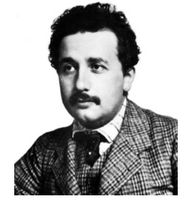
\includegraphics[width=0.2\textwidth]{pictures/Einestin.png}
    \end{center}
    
\end{rightcolumn}
   
\end{paracol}

\textbf{Hubble discovers other galaxies and Hubble's Law in 1922 and 1929}
\columnratio{0.6, 0.4}
\begin{paracol}{2}
    \begin{leftcolumn}
        He discovered:
        \begin{itemize}
            \item[!] All galaxies were moving \blue{away} from us
            \item[!] All galaxies are \blue{Redshift}
            \item[!] Back to the past, the galaxies would all be \blue{closer} together. There must be a time when all the galaxies \blue{overlap}. This time happened 11.8 billions years ago. This is considered the age of the universe.
        \end{itemize}
    \end{leftcolumn}

    \begin{rightcolumn}
        \begin{center}
            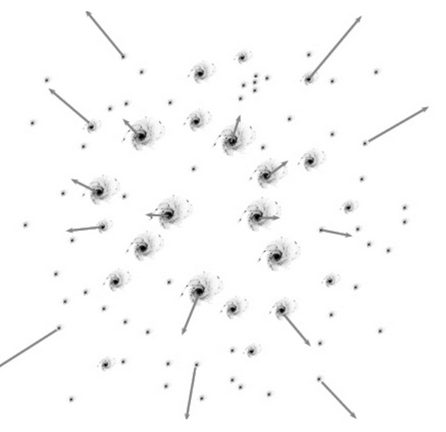
\includegraphics[width=0.3\textwidth]{pictures/hubble.png}
        \end{center}
    \end{rightcolumn}
\end{paracol}

\newpage
\textbf{Alpher and Gamow calculate cosmic abundances in 1948} \\

Alpher and Gamow assumed that the early universe was very \blue{hot} and calculate the \blue{abundance of certain elements} (other than hydrogen) during the early stages of the universe.

\begin{center}
    Helium - 25\% \\
    Deuterium - 0.001\% \\
    Lithium - 0.00000001\%
\end{center}

This predictions were confirmed by observational evidences
\begin{greenblock}
    \begin{worddef}{The theory}
        became known ass \blue{Big Bang Nuclear Synthesis}
    \end{worddef}
\end{greenblock}

\textbf{Cosmic microwave background (CMB) was discovered in 1964}\\

While trying building a telescope, Penzias and Wilson, accidentally discovered that there was a signal came from every direction
in the sky. The signal has the same frequency as \blue{microwave} and a temperature about \blue{2.7 degrees kelvin}.\\

The ssignal was latter interpreted to be the \red{light} from the \red{early stages of universe}.\\
It's the first light ever emitted from the Big Bang.\\

\textbf{Singularity Theorems in 1968}\\

\red{Roger Penrose} and \red{Stephen Hawking} proved mathematically that the universe must have started with a \red{singularity}\\

The means there was a \red{beginning to the time itself}